% Classe do documento e parâmetros gerais.
\documentclass[a4paper,openright,twoside,11pt]{report}

%
% Times New Roman font.
%
\usefont{T1}{ptm}{m}{n}
\selectfont

% Packages a utilizar e respetivos parâmetros.
\usepackage[utf8]{inputenc}
\usepackage[portuguese]{babel}
\addto{\captionsportuguese}{\renewcommand{\bibname}{Refer\^{e}ncias}}
\addto{\captionsportuguese}{\renewcommand{\contentsname}{\'Indice}}
\addto{\captionsportuguese}{\renewcommand{\appendixname}{Anexo}}
\usepackage{graphicx}
\usepackage{url}
\usepackage[Algoritmo]{algorithm}
\usepackage{algorithmicx}
\usepackage{algpseudocode}
\usepackage{indentfirst}

\renewcommand{\algorithmicrequire}{\textbf{Dados: }}
\renewcommand{\algorithmicensure}{\textbf{Resultado: }}

% Definições das dimensões das páginas
\setlength{\textheight}{24.00cm}
\setlength{\textwidth}{15.50cm}
\setlength{\topmargin}{0.35cm}
\setlength{\headheight}{0cm}
\setlength{\headsep}{0cm}
\setlength{\oddsidemargin}{0.25cm}
\setlength{\evensidemargin}{0.25cm}

%
% Times New Roman font.
%
\usefont{T1}{ptm}{m}{n}
\selectfont


%\renewcommand{\baselinestretch}{1}

%
% Página inicial (capa)
%
\title{
   \vspace{-60mm}
   \begin{minipage}[l]{160mm}
   	\resizebox{50mm}{!}{
\includegraphics{./figures/logoISEL.png}}\\
   \end{minipage}\\
   \vspace{20mm}
   % Título do projeto na forma capitalizada. A primeira letra de cada palavra deve ser maiúscula.
   {\bf Gestão Inteligente de Stocks}
}

% Nome dos autores (um por linha)
\author{
	\begin{tabular}{ll}
		& 42142 \hspace{0.1cm} Ana Santos, \hspace{0.3cm} 42142@alunos.isel.ipl.pt, \hspace{0.1cm} 967064568\\
		& 42162 \hspace{0.1cm} Inês Soares, \hspace{0.35cm} 42162@alunos.isel.ipl.pt, \hspace{0.1cm} 914182857\\
		& 42181 \hspace{0.1cm} Nuno Veloso, \hspace{0.1cm} 42181@alunos.isel.ipl.pt, \hspace{0.1cm} 910364327\\
	\end{tabular}
}


\date{
	\vspace{80mm}
	\begin{tabular}{ll}
		{Orientadores} & Matilde Pato, \hspace{0.1cm}mpato@deetc.isel.pt\\
		& Nuno Datia, \hspace{0.37cm}datia@isel.ipl.pt\\
	\end{tabular}\\
	% Deixar o indicador respetivo em função da versão do relatório.
	\vspace{10mm}
	Relatório de progresso realizado no âmbito de Projeto e Seminário,\\
	do curso de licenciatura em Engenharia Informática e de Computadores\\
	Semestre de Verão 2017/2018\\
	\vspace{20mm}
	Março de 2018
}

\begin{document}

\pagenumbering{roman}
\thispagestyle{empty}
\maketitle

\baselineskip 18pt % line spacing: 12pt for single, 18pt for 1 1/2, and 24pt for double spacing

\newpage
\thispagestyle{empty}
% Fim da contracapa

% Página com identificação completa (número e nome) e assinaturas dos estudante(s) e do(s) orientador(es)
\cleardoublepage\newpage
\setcounter{page}{1}
\begin{center}
{\Large\bf Instituto Superior de Engenharia de Lisboa}\\
{\large Licenciatura em Engenharia Informática e de Computadores}\\
%Projecto e Seminário\\
\vspace{50mm}
{\large \bf  Gestão Inteligente de Stocks}\\
\vspace{20mm}
\begin{tabular}{rl}
  42142 & Ana Rita Ferreira dos Santos\\
  42162 & Inês Lima Amil Soares\\
  42181 & Nuno Manuel Olival Veloso\\
\end{tabular}\\
\vspace{8mm}
\noindent\rule{12cm}{0.6pt}\\
\vspace{10mm}
\noindent\rule{12cm}{0.6pt}\\
\vspace{10mm}
\begin{tabular}{rl}
  Orientadores: & Nuno Miguel Soares Datia\\   
                & Matilde Pós-de-Mina Pato\\
\end{tabular}\\
\vspace{8mm}
\noindent\rule{12cm}{0.6pt}\\
\vspace{10mm}
\noindent\rule{12cm}{0.6pt}\\
\vspace{15mm}
Relatório de progresso realizado no âmbito de Projeto e Seminário,\\
do curso de licenciatura em Engenharia Informática e de Computadores\\
Semestre de Verão 2017/2018\\
\vspace{20mm}
Março de 2018\\
\end{center}

% Página de resumo em Português
\cleardoublepage\newpage
\chapter*{Resumo}
Texto do resumo.\\

Breve descrição do projecto, dos resultados importantes e das conclusões: o objectivo é dar ao leitor uma visão global do projecto (não deve exceder uma página). 

{\bf Palavras-chave:} lista de palavras-chave, ordenadas alfabeticamente, separadas por ;.

% Página de resumo em Inglês
\cleardoublepage\newpage
\chapter*{Abstract}
Abstract text (1 page).\\

{\bf Keywords:} sorted keyword list, delimited by ;.

% Página de agradecimentos
\cleardoublepage\newpage
\chapter*{Agradecimentos}
Texto dos agradecimentos. É opcional.\\

% Geração do índice de conteúdos
\cleardoublepage\newpage
\tableofcontents
\cleardoublepage

% Geração do índice de figuras
\listoffigures
\cleardoublepage

% Geração do índice de tabelas
\listoftables
\cleardoublepage

% Iniciar a numeração de páginas
\setcounter{page}{1}
\pagenumbering{arabic}

% Capitulo 1
%%
% Capítulo 1
%
\chapter{Introdução} \label{cap1}

A gestão de stocks é um processo estruturado, assim, no âmbito da \acrfull{iot} e de forma a simplificar o quotidiano de cada um, surge este projeto. Atualmente, são várias as aplicações responsáveis por fornecer listas de compras, porém carecem de controlo de stocks e conhecimento dos hábitos dos seus utilizadores. A aplicação desenvolvida neste projeto distingue-se pela elaboração/presença de um algoritmo de previsão de stocks, com base no histórico de consumo e reposição do utilizador.

%
% Secção 1.1
%
\section{Enquadramento} \label{sec11}

No contexto do projeto assume-se a existência de duas formas de apresentação para os produtos: avulsos e embalados. Os primeiros são conservados em sistemas de arrumação marcados com \textit{tags} programáveis por \textit{smartphones}. Os detalhes dos produtos são especificados pelo utilizador e carregados para a \textit{tag}. Enquanto que para os produtos embalados, admite-se que os produtores utilizam \textit{tags}, \acrfull{nfc} ou \acrfull{rfid}, para guardar os rótulos de forma digital e em formato standard.

Após a aquisição, os produtos são armazenados em locais que devem dispor de dispositivos de hardware equipados com leitores de \textit{tags}. É recolhida a informação presente na \textit{tag}, identificado o tipo de movimento (entrada ou saída) e enviado para a \gls{api-web}. 

Através da aplicação disponibilizada, o utilizador poderá consultar:
\begin{itemize} \itemsep 0pt
	\item os produtos em stock,
	\item as listas do sistema e/ou as por si criadas,
	\item as suas casas e caraterísticas,
	\item as alergias dos membros de cada casa,
	\item os locais de armazenamento e dispositivos de hardware.
\end{itemize}

Será ainda possível:
\begin{itemize} \itemsep 0pt
	\item receber alertas de produtos perto do fim da validade,
	\item especificar stocks mínimos e/ou indesejados,
	\item partilhar listas entre utilizadores da mesma casa.
\end{itemize}

%
% Secção 1.2
%
\section{Metas e Objetivos} \label{sec12}
Têm-se como objetivos, os seguintes pontos:
\begin{itemize} \itemsep 0pt
	\item Desenho das Aplicações Móvel e Web
	\item Desenvolvimento da \gls{api-web}
	\item Elaboração do Algoritmo de Previsão de Stocks
\end{itemize}


%
% Secção 1.3
%
\section{Especificações do Projecto e Resumo da Solução} \label{sec13}

O projeto é composto por 2 blocos principais, que se relacionam. A Figura \ref{esquema_geral} representa esses blocos. 

\textit(Figura Aqui)

Um dos blocos é a interação com o utilizador, através de duas aplicações, uma móvel e uma Web. A aplicação móvel desenvolvida apenas para a plataforma \textit{Android}, e utilizando a linguagem \textit{Kotlin}. Para a aplicação Web, implementada recorrendo à linguagem \textit{JavaScript}, com o auxilio da \textit{framework Express}. 

O outro bloco é a \gls{api-web} desenvolvida com a \textit{framework} da \textit{Spring}, chamada de \textit{Spring Boot}. Subjacente a este último bloco estão as camadas: \acrfull{db}, \acrfull{dal}, \acrfull{bll}.  A camada da base de dados (\acrshort{db}), realizada com o \acrfull{sgdb} \textit{PostgreSQL}. Para a camada de acesso a dados (\acrshort{dal}), responsável pelas leituras e escritas, a ferramenta utilizada é a linguagem de programação \textit{Java}, com a \gls{api} \acrfull{jdbc}. A camada da lógica de negócio (\acrshort{bll}), também se serve da ferramenta mencionada anterior para a sua implementação, esta camada é responsável pela gestão dos dados obtidos da \acrshort{db} ou da \gls{api-web}.


%
% Secção 1.4
%
\section{Estrutura do Relatório} \label{sec14}
O relatório está estruturado em X capítulos.

O capítulo 2.


% Capitulo 2
%%
% Capítulo 2
%
\chapter{Gestão de Stocks} \label{cap2}

Neste capítulo a aplicação Smart Stocks é descrita na secção \ref{sec21}, bem como os requisitos funcionais e opcionais na secção \ref{sec22}.


%
% Secção 2.1
%
\section{Aplicação Smart Stocks} \label{sec21}
A Smart Stocks é uma aplicação que visa dar suporte à gestão de stocks domésticos. Com fim de se alcançar o desejado é necessário recolher determinadas informações, tais como, as características da casa a gerir, as particularidades dos membros co-habitantes da casa e ainda os padrões de consumo e reposição. Para facilitar tal tarefa são disponibilizadas listas geridas pelo sistema. Por exemplo, lista de compras e lista dos itens em stock na casa, cuja consistência é garantida às custas dos movimentos de entrada e saída dos itens nos diversos locais de armazenamento.

Em seguida listam-se as diversas entidades que compõem o sistema de informação que permita gerir os itens em stock numa dada casa.
\subsubsection{Casa}
\begin{itemize}
	\item Cada casa é caracterizada por um identificador único, um nome, atribuído por um utilizador no momento de registo da casa. O número de bebés, crianças, adultos e seniores que vivem nessa casa.
	\item Uma casa está associada a um ou mais utilizadores, podendo um utilizador ter várias casas. 
	\item Podem existir um ou mais administradores.
	\item A casa pode ter vários itens em stock presentes na mesma.
	\item Para cada casa existem vários locais de armazenamento dos itens, por exemplo armários, frigoríficos, etc.
	\item Em cada casa deve ser possível conhecer as alergias assim como quantos membros possuem essa alergia (os membros não precisam necessariamente de estar registados).
\end{itemize}

\subsubsection{Utilizador}
\begin{itemize}
	\item Uma pessoa é representada por um utilizador que é identificado univocamente por um email ou por um nome de utilizador, pelo nome da pessoa, a sua idade e uma password.
\end{itemize}

\subsubsection{Listas}
\begin{itemize}
	\item Cada lista é composta por um identificador único e um nome.
	\item Uma lista pode ter vários produtos.
	\item Existem dois tipos de listas: de sistema e de utilizador. 
	\item As listas de sistema são comuns a todos os utilizadores registados, contudo são particulares a cada casa. 
	\item Um utilizador pode criar as suas listas, partilhando-as com outros utilizadores da casa ou tornar a lista secreta.
\end{itemize}

\subsubsection{Categoria}
\begin{itemize}
	\item Uma categoria é identificada univocamente por um número ou por um nome.
\end{itemize}


\subsubsection{Produtos}
\begin{itemize}
	\item Um produto é constituído por um identificador único, um nome, se é ou não comestível, e a validade perecível.
	\item Para os produtos presentes numa lista pode ser possível saber a sua marca e a quantidade.
	\item Um produto pertence a uma categoria, podendo uma categoria ter vários produtos.
	\item Um produto pode ser concretizado por diversos itens em stock na casa.
\end{itemize}
 
\subsubsection{Item em Stock}
\begin{itemize}
	\item Um item em stock é a concretização de um produto que existe numa casa. É identificado univocamente por um número ou por uma marca, uma variedade e um segmento, é também caracterizado por uma descrição, o local de conservação, a quantidade e as datas de validade. 
	\item Para cada item deve ser possível saber os seus movimentos de entrada e saída de um local de armazenamento.
	\item Deve também ser possível saber os alergénios de um item presente na casa.
\end{itemize}

\subsubsection{Movimento}
\begin{itemize}
	\item Para cada movimento deve ser possível saber o tipo do movimento (entrada ou saída), a data em que ocorreu e a quantidade de produtos. 
\end{itemize}

\subsubsection{Local de armazenamento}
\begin{itemize}
	\item Cada local de armazenamento é caraterizado por um identificador único, a temperatura e um nome.
	\item Deve ser possível saber a quantidade de cada item presente no local.
	\item Um local de armazenamento pode ter vários itens em stock presentes na casa e estar associado a diversos movimentos.
\end{itemize}


%
% Secção 2.2
%
\section{Requisitos Funcionais e Opcionais} \label{sec22}

\paragraph{Requisitos Funcionais}
\begin{itemize}
	\item Informar o utilizador dos produtos existentes, a sua validade e a sua quantidade;
	\item Alertas sobre os produtos que estão perto da data de validade;
	\item Geração da lista de compras com os produtos em falta;
	\item Possibilidade de especificar os produtos a ter sempre em stock bem como as suas quantidades mínimas;	
	\item Lista de Compras \textit{Offline};
	\item Listas partilhadas entre utilizadores da mesma casa;
	\item Criação de Listas;
	\item Especificação das alergias dos membros da casa.
\end{itemize}


\paragraph{Requisitos Opcionais}
\begin{itemize}
	\item Lista de produtos quase a expirar;
	\item Lista de produtos indesejados (Lista Negra);
	\item Lista de contenção em situações de emergência (Lista SOS);
	\item Inserir refeições extraordinárias de eventos a realizar num futuro próximo, para acrescentar alimentos não básicos à lista de compras;
\end{itemize}


%
% Secção 2.3
%
\section{Dificuldades Encontradas} \label{sec23}

Para a realização deste projeto encontrámos dificuldades nos aspetos a seguir referidos.

\subsection{Rótulos em Formato Não Digital}

Nos dias de hoje, os produtos não possuem rótulos digitais. Isto é um problema para a concretização do projeto, na medida em que se torna menos eficiente a recolha dos dados presentes nos produtos. Contudo, assumindo que este problema é resolvido fora do âmbito do projeto, apenas é preciso definir um formato standard de como os dados devem ser armazenados nas \textit{tags}, que podem ser \acrshort{nfc} ou \acrshort{rfid}. Num cenário ideal, este formato deve ser respeitado por todos os embaladores. Assim, os produtos têm um rótulo, código de barras e uma \textit{tag} \acrshort{nfc} ou \acrshort{rfid}, com a informação necessária. Está fora do âmbito do trabalho implementar o suporte hardware para a leitura das \textit{tags} e qual o sentido do movimento (entrada ou saída). Assume-se que essas informações são disponibilizadas num formato conhecido. 


\subsection{Ausência de Identificador Único nos Itens}

Os itens não dispõem de um identificador unívoco. Alguns deles contêm um lote e um número de série. A ausência deste identificador impede a distinção entre itens iguais, o que impossibilita saber se entrou um novo item no local de armazenamento ou se saiu um dos itens presentes. Tal facto torna a gestão dos stocks dependente do dispositivo de hardware para distinguir o tipo de movimento.

% Capitulo 3
%%
% Capítulo 3
%
\chapter{Solução Proposta} \label{cap3}

%
% Modelo de Dados
%
\section{Modelo de Dados}\label{sec35}






% Modelo EA
\subsection{Modelo Entidade-Associação}\label{subsec311}

\begin{figure}[H]
	\hspace*{-2,5cm}
	\centering
	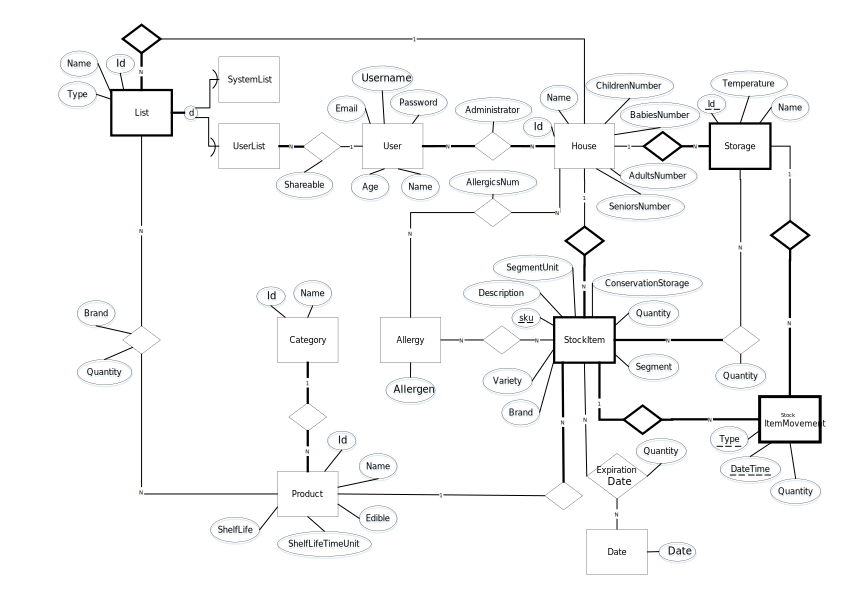
\includegraphics[width=20cm,height=15cm,scale=1]{./files/EA.pdf}
	\caption{Modelo Entidade-Associação}
	\label{modelo-ea}
\end{figure}

% Domínio dos Atributos
\subsection{Domínio dos Atributos}\label{subsec313}
\raggedbottom
% House
\begin{table} [H]
	\centering
	\caption{Domínio dos Atributos da Entidade House.} \vspace{2mm}
	\label{tab-dominio-atributos-house}
	\resizebox{\textwidth}{!}{%
		\begin{tabular}{|c|c|C{2.5cm}|C{2.7cm}|C{3.6cm}|C{2.3cm}|}
			\hline
			\textbf{Entidade} & \textbf{Atributo} & \textbf{Domínio} & \textbf{Tipo Variável (PostgreSQL)} & \textbf{Restrições} & \textbf{Nullable}\\ \hline
			\multirow{6}{*}{House} & house\_id & Número inteiro auto-incrementado & bigserial & - & não\\ \cline{2-6}
			& house\_name & Cadeia de caracteres de comprimento variável & character varying(35) & até 35 caracteres & não\\ \cline{2-6}
			& house\_characteristics & Objeto \acrshort{json} & json & - & não\\ \hline
		\end{tabular}
	}
\end{table}

% User
\begin{table} [H]
	\centering
	\caption{Domínio dos Atributos da Entidade User.} \vspace{2mm}
	\label{tab-dominio-atributos-user}
	\resizebox{\textwidth}{!}{%
		\begin{tabular}{|c|c|C{2.5cm}|C{2.7cm}|C{3.6cm}|C{2.3cm}|}
			\hline
			\textbf{Entidade} & \textbf{Atributo} & \textbf{Domínio} & \textbf{Tipo Variável (PostgreSQL)} & \textbf{Restrições} & \textbf{Nullable}\\ \hline
			\multirow{5}{*}{User} & user\_username & Cadeia de caracteres de comprimento variável & character varying(30) & até 30 caracteres & não\\ \cline{2-6}
			& user\_email & Cadeia de caracteres de comprimento variável & character varying(254) & até 254 caracteres & não\\ \cline{2-6}
			& user\_age & Número inteiro & smallint & user\_age in [0, 150] & não\\ \cline{2-6}
			& user\_name & Cadeia de caracteres de comprimento variável & character varying(70) & até 70 caracteres & não\\ \cline{2-6}
			& user\_password & Cadeia de caracteres de comprimento variável & character varying(50) & até 50 caracteres & não\\ \hline
		\end{tabular}
	}
\end{table}

% Allergy
\begin{table} [H]
	\centering
	\caption{Domínio dos Atributos da Entidade Allergy.} \vspace{2mm}
	\label{tab-dominio-atributos-allergy}
	\resizebox{\textwidth}{!}{%
		\begin{tabular}{|c|c|C{2.5cm}|C{2.7cm}|C{3.6cm}|C{2.3cm}|}
			\hline
			\textbf{Entidade} & \textbf{Atributo} & \textbf{Domínio} & \textbf{Tipo Variável (PostgreSQL)} & \textbf{Restrições} & \textbf{Nullable}\\ \hline
			{Allergy} & allergy\_allergen & Cadeia de caracteres de comprimento variável & character varying(75) & até 75 caracteres & não\\ \hline
		\end{tabular}
	}
\end{table}


% Recipe
\begin{table} [H]
	\centering
	\caption{Domínio dos Atributos da Entidade Recipe.} \vspace{2mm}
	\label{tab-dominio-atributos-recipe}
	\resizebox{\textwidth}{!}{%
		\begin{tabular}{|c|c|C{2.5cm}|C{2.7cm}|C{3.6cm}|C{2.3cm}|}
			\hline
			\textbf{Entidade} & \textbf{Atributo} & \textbf{Domínio} & \textbf{Tipo Variável (PostgreSQL)} & \textbf{Restrições} & \textbf{Nullable}\\ \hline
			\multirow{9}{*}{Recipe} & recipe\_id & Número inteiro auto-incrementado & bigserial & - & não\\ \cline{2-6}
			& recipe\_name & Cadeia de caracteres de comprimento variável & character varying(35) & até 35 caracteres & não\\ \cline{2-6}
			& recipe\_instructions & Cadeia de caracteres de comprimento variável & text & - & não\\ \cline{2-6}
			& recipe\_difficulty & Cadeia de caracteres de comprimento variável & character varying(9) & recipe\_difficulty in ['easy', 'average', 'difficult'] & sim\\ \cline{2-6}
			& recipe\_time & Número inteiro & smallint & recipe\_time \textgreater{} 0 & sim\\ \cline{2-6}
			& recipe\_servings & Número inteiro & smallint & recipe\_servings \textgreater{} 0 & sim\\ \cline{2-6}
			& recipe\_cuisine & Cadeia de caracteres de comprimento variável & character varying(35) & até 35 caracteres & sim\\ \cline{2-6}
			& recipe\_dishType & Cadeia de caracteres de comprimento variável & character varying(35) & até 35 caracteres & sim\\ \cline{2-6}
			& recipe\_type & Cadeia de caracteres de comprimento variável & character varying(7) & recipe\_type  in ['system', 'user'] & não\\ \hline
		\end{tabular}
	}
\end{table}

% System Recipe
\begin{table} [H]
	\centering
	\caption{Domínio dos Atributos da Entidade SystemRecipe.} \vspace{2mm}
	\label{tab-dominio-atributos-systemRecipe}
	\resizebox{\textwidth}{!}{%
		\begin{tabular}{|c|c|C{2.5cm}|C{2.7cm}|C{3.6cm}|C{2.3cm}|}
			\hline
			\textbf{Entidade} & \textbf{Atributo} & \textbf{Domínio} & \textbf{Tipo Variável (PostgreSQL)} & \textbf{Restrições} & \textbf{Nullable}\\ \hline
			{System Recipe} & recipe\_id & Número inteiro & bigint & recipe\_id \textgreater{} 0 & não\\ \hline
		\end{tabular}
	}
\end{table}

% User Recipe
\begin{table} [H]
	\centering
	\caption{Domínio dos Atributos da Entidade UserRecipe.} \vspace{2mm}
	\label{tab-dominio-atributos-userRecipe}
	\resizebox{\textwidth}{!}{%
		\begin{tabular}{|c|c|C{2.5cm}|C{2.7cm}|C{3.6cm}|C{2.3cm}|}
			\hline
			\textbf{Entidade} & \textbf{Atributo} & \textbf{Domínio} & \textbf{Tipo Variável (PostgreSQL)} & \textbf{Restrições} & \textbf{Nullable}\\ \hline
			\multirow{2}{*}{User Recipe} & recipe\_id & Número inteiro & bigint & recipe\_id \textgreater{} 0 & não\\ \cline{2-6}
			& user\_username & Cadeia de caracteres de comprimento variável & character varying(30) & até 30 caracteres & não\\ \hline
		\end{tabular}
	}
\end{table}

% Shared Recipe
\begin{table} [H]
	\centering
	\caption{Domínio dos Atributos da Entidade SharedRecipe.} \vspace{2mm}
	\label{tab-dominio-atributos-sharedRecipe}
	\resizebox{\textwidth}{!}{%
		\begin{tabular}{|c|c|C{2.5cm}|C{2.7cm}|C{3.6cm}|C{2.3cm}|}
			\hline
			\textbf{Entidade} & \textbf{Atributo} & \textbf{Domínio} & \textbf{Tipo Variável (PostgreSQL)} & \textbf{Restrições} & \textbf{Nullable}\\ \hline
			\multirow{2}{*}{Shared Recipe} & recipe\_id & Número inteiro & bigint & recipe\_id \textgreater{} 0 & não\\ \cline{2-6}
			& user\_username & Cadeia de caracteres de comprimento variável & character varying(30) & até 30 caracteres & não\\ \hline
		\end{tabular}
	}
\end{table}

% List
\begin{table} [H]
	\centering
	\caption{Domínio dos Atributos da Entidade List.} \vspace{2mm}
	\label{tab-dominio-atributos-list}
	\resizebox{\textwidth}{!}{%
		\begin{tabular}{|c|c|C{2.5cm}|C{2.7cm}|C{3.6cm}|C{2.3cm}|}
			\hline
			\textbf{Entidade} & \textbf{Atributo} & \textbf{Domínio} & \textbf{Tipo Variável (PostgreSQL)} & \textbf{Restrições} & \textbf{Nullable}\\ \hline
			\multirow{4}{*}{List} & house\_id & Número inteiro & bigint & house\_id \textgreater{} 0 & não\\ \cline{2-6}
			& list\_id & Número inteiro auto-incrementado & smallint & - & não\\ \cline{2-6}
			& list\_name & Cadeia de caracteres de comprimento variável & character varying(35) & até 35 caracteres & não\\ \cline{2-6}
			& list\_type & Cadeia de caracteres de comprimento variável & character varying(7) & list\_type  in ['system', 'user'] & não\\ \hline
		\end{tabular}
	}
\end{table}

% System List
\begin{table} [H]
	\centering
	\caption{Domínio dos Atributos da Entidade SystemList.} \vspace{2mm}
	\label{tab-dominio-atributos-systemList}
	\resizebox{\textwidth}{!}{%
		\begin{tabular}{|c|c|C{2.5cm}|C{2.7cm}|C{3.6cm}|C{2.3cm}|}
			\hline
			\textbf{Entidade} & \textbf{Atributo} & \textbf{Domínio} & \textbf{Tipo Variável (PostgreSQL)} & \textbf{Restrições} & \textbf{Nullable}\\ \hline
			\multirow{2}{*}{System List} & house\_id & Número inteiro & bigint & house\_id \textgreater{} 0 & não\\ \cline{2-6}
			& list\_id & Número inteiro & smallint & list\_id \textgreater{} 0 & não\\ \hline
		\end{tabular}
	}
\end{table}

% User List
\begin{table} [H]
	\centering
	\caption{Domínio dos Atributos da Entidade UserList.} \vspace{2mm}
	\label{tab-dominio-atributos-userList}
	\resizebox{\textwidth}{!}{%
		\begin{tabular}{|c|c|C{2.5cm}|C{2.7cm}|C{3.6cm}|C{2.3cm}|}
			\hline
			\textbf{Entidade} & \textbf{Atributo} & \textbf{Domínio} & \textbf{Tipo Variável (PostgreSQL)} & \textbf{Restrições} & \textbf{Nullable}\\ \hline
			\multirow{4}{*}{User List} & house\_id & Número inteiro & bigint & house\_id \textgreater{} 0 & não\\ \cline{2-6}
			& list\_id & Número inteiro & smallint & list\_id \textgreater{} 0 & não\\ \cline{2-6}
			& user\_username & Cadeia de caracteres de comprimento variável & character varying(30) & até 30 caracteres & não\\ \cline{2-6}
			& list\_shareable & Booleano & boolean & - & sim\\ \hline
		\end{tabular}
	}
\end{table}

% Category
\begin{table} [H]
	\centering
	\caption{Domínio dos Atributos da Entidade Category.} \vspace{2mm}
	\label{tab-dominio-atributos-category}
	\resizebox{\textwidth}{!}{%
		\begin{tabular}{|c|c|C{2.5cm}|C{2.7cm}|C{3.6cm}|C{2.3cm}|}
			\hline
			\textbf{Entidade} & \textbf{Atributo} & \textbf{Domínio} & \textbf{Tipo Variável (PostgreSQL)} & \textbf{Restrições} & \textbf{Nullable}\\ \hline
			\multirow{2}{*}{Category} & category\_id & Número inteiro auto-incrementado & serial & - & não\\ \cline{2-6}
			& category\_name & Cadeia de caracteres de comprimento variável & character varying(35) & até 35 caracteres & não\\ \hline
		\end{tabular}
	}
\end{table}

% Product
\begin{table} [H]
	\centering
	\caption{Domínio dos Atributos da Entidade Product.} \vspace{2mm}
	\label{tab-dominio-atributos-product}
	\resizebox{\textwidth}{!}{%
		\begin{tabular}{|c|c|C{2.5cm}|C{2.7cm}|C{3.8cm}|C{2cm}|}
			\hline
			\textbf{Entidade} & \textbf{Atributo} & \textbf{Domínio} & \textbf{Tipo Variável (PostgreSQL)} & \textbf{Restrições} & \textbf{Nullable}\\ \hline
			\multirow{6}{*}{Product} & category\_id & Número inteiro & integer & category\_id \textgreater{} 0 & não\\ \cline{2-6}
			& product\_id & Número inteiro auto-incrementado & integer & - & não\\ \cline{2-6}
			& product\_name & Cadeia de caracteres de comprimento variável & character varying(35) & até 35 caracteres & não\\ \cline{2-6}
			& product\_edible & Booleano & boolean & - & não\\ \cline{2-6}
			& product\_shelfLife & Número inteiro & smallint & product\_shelfLife \textgreater{} 0 & não\\ \cline{2-6}
			& product\_shelfLifeTimeUnit & Cadeia de caracteres de comprimento variável & character varying(5) & product\_shelfLifeTimeUnit in ['day', 'week', 'month', 'year'] & não\\ \hline
		\end{tabular}
	}
\end{table}

% StockItem
\begin{table} [H]
	\centering
	\caption{Domínio dos Atributos da Entidade StockItem.} \vspace{2mm}
	\label{tab-dominio-atributos-stockItem}
	\resizebox{\textwidth}{!}{%
		\begin{tabular}{|c|c|C{2.5cm}|C{2.7cm}|C{3.6cm}|C{2cm}|}
			\hline
			\textbf{Entidade} & \textbf{Atributo} & \textbf{Domínio} & \textbf{Tipo Variável (PostgreSQL)} & \textbf{Restrições} & \textbf{Nullable}\\ \hline
			\multirow{11}{*}{StockItem} & house\_id & Número inteiro & bigint & house\_id \textgreater{} 0 & não\\ \cline{2-6}
			& stockItem\_sku & Cadeia de caracteres de comprimento variável & character varying(128) & até 128 caracteres & não\\ \cline{2-6}
			& category\_id & Número inteiro & integer & category\_id \textgreater{} 0 & não\\ \cline{2-6}
			& product\_id & Número inteiro & integer & product\_id \textgreater{} 0 & não\\ \cline{2-6}
			& stockItem\_brand & Cadeia de caracteres de comprimento variável & character varying(35) & até 35 caracteres & não\\ \cline{2-6}
			& stockItem\_segment & Número décimal & real & stockItem\_segment \textgreater{} 0 & não\\ \cline{2-6}
			& stockItem\_variety & Cadeia de caracteres de comprimento variável & character varying(35) & até 35 caracteres & não\\ \cline{2-6}
			& stockItem\_quantity & Número inteiro & smallint & stockItem\_quantity \textgreater{} 0 & não\\ \cline{2-6}
			& stockItem\_segmentUnit & Cadeia de caracteres de comprimento variável & character varying(5) & stockItem\_segmentUnit in ['kg', 'dag', 'hg', 'g', 'dg', 'cg', 'mg', 'kl', 'hl', 'dal', 'l', 'dl', 'cl', 'ml', 'oz', 'lb', 'pt', 'fl oz', 'units'] & não\\ \cline{2-6}
			& stockItem\_description & Cadeia de caracteres de comprimento variável & text & - & sim\\ \cline{2-6}
			& stockItem\_conservationStorage & Cadeia de caracteres de comprimento variável & character varying(128) & até 128 caracteres & não\\ \hline
		\end{tabular}
	}
\end{table}
	
% Ingredient
\begin{table} [H]
	\centering
	\caption{Domínio dos Atributos da Entidade Ingredient.} \vspace{2mm}
	\label{tab-dominio-atributos-ingredient}
	\resizebox{\textwidth}{!}{%
		\begin{tabular}{|c|c|C{2.5cm}|C{2.7cm}|C{3.6cm}|C{2.3cm}|}
			\hline
			\textbf{Entidade} & \textbf{Atributo} & \textbf{Domínio} & \textbf{Tipo Variável (PostgreSQL)} & \textbf{Restrições} & \textbf{Nullable}\\ \hline
			\multirow{5}{*}{Ingredient} & recipe\_id & Número inteiro & integer & recipe\_id \textgreater{} 0 & não\\ \cline{2-6}
			& category\_id & Número inteiro & integer & category\_id \textgreater{} 0 & não\\ \cline{2-6}
			& product\_id & Número inteiro & integer & product\_id \textgreater{} 0 & não\\ \cline{2-6}
			& ingredient\_quantity & Número inteiro & integer & ingredient\_quantity \textgreater{} 0 & não\\ \cline{2-6}
			& ingredient\_quantityUnit & Cadeia de caracteres de comprimento variável & character varying(5) & ingredient\_quantityUnit in ['kg', 'dag', 'hg', 'g', 'dg', 'cg', 'mg', 'kl', 'hl', 'dal', 'l', 'dl', 'cl', 'ml', 'oz', 'lb', 'pt', 'fl oz', 'units'] & não\\ \hline
		\end{tabular}
	}
\end{table}

% Storage
\begin{table} [H]
	\centering
	\caption{Domínio dos Atributos da Entidade Storage.} \vspace{2mm}
	\label{tab-dominio-atributos-storage}
	\resizebox{\textwidth}{!}{%
		\begin{tabular}{|c|c|C{2.5cm}|C{2.7cm}|C{3.6cm}|C{2.3cm}|}
			\hline
			\textbf{Entidade} & \textbf{Atributo} & \textbf{Domínio} & \textbf{Tipo Variável (PostgreSQL)} & \textbf{Restrições} & \textbf{Nullable}\\ \hline
			\multirow{4}{*}{Storage} & house\_id & Número inteiro & bigint & house\_id \textgreater{} 0 & não\\ \cline{2-6}
			& storage\_id & Número inteiro auto-incrementado & smallint & - & não\\ \cline{2-6}
			& storage\_name & Cadeia de caracteres de comprimento variável & character varying(35) & até 35 caracteres & não\\ \cline{2-6}
			& storage\_temperature & Intervalo de números decimais & numrange & - & não\\ \hline
		\end{tabular}
	}
\end{table}

% User House
\begin{table} [H]
	\centering
	\caption{Domínio dos Atributos da Entidade UserHouse.} \vspace{2mm}
	\label{tab-dominio-atributos-userHouse}
	\resizebox{\textwidth}{!}{%
		\begin{tabular}{|c|c|C{2.5cm}|C{2.7cm}|C{3.6cm}|C{2.3cm}|}
			\hline
			\textbf{Entidade} & \textbf{Atributo} & \textbf{Domínio} & \textbf{Tipo Variável (PostgreSQL)} & \textbf{Restrições} & \textbf{Nullable}\\ \hline
			\multirow{3}{*}{UserHouse} & house\_id & Número inteiro & bigint & house\_id \textgreater{} 0 & não\\ \cline{2-6}
			& user\_username & Cadeia de caracteres de comprimento variável & character varying(30) & até 30 caracteres & não\\ \cline{2-6}
			& userHouse\_administrator & Booleano & boolean & - & sim\\ \hline
		\end{tabular}
	}
\end{table}

% StockItem Storage
\begin{table} [H]
	\centering
	\caption{Domínio dos Atributos da Entidade StockItemStorage.} \vspace{2mm}
	\label{tab-dominio-atributos-stockItemStorage}
	\resizebox{\textwidth}{!}{%
		\begin{tabular}{|c|c|C{2.3cm}|C{2.7cm}|C{3.6cm}|C{2cm}|}
			\hline
			\textbf{Entidade} & \textbf{Atributo} & \textbf{Domínio} & \textbf{Tipo Variável (PostgreSQL)} & \textbf{Restrições} & \textbf{Nullable}\\ \hline
			\multirow{4}{*}{StockItemStorage} & house\_id & Número inteiro & bigint & house\_id \textgreater{} 0 & não\\ \cline{2-6}
			& stockItem\_sku & Cadeia de caracteres de comprimento variável & character varying(128) & até 128 caracteres & não\\ \cline{2-6}
			& storage\_id & Número inteiro & smallint & storage\_id \textgreater{} 0 & não\\ \cline{2-6}
			& stockItemStorage\_quantity & Número inteiro & smallint & stockItemStorage\_quantity \textgreater{} 0 & não\\ \hline
		\end{tabular}
	}
\end{table}

% StockItem Movement
\begin{table} [H]
	\centering
	\caption{Domínio dos Atributos da Entidade StockItemMovement.} \vspace{2mm}
	\label{tab-dominio-atributos-stockItemMovement}
	\resizebox{\textwidth}{!}{%
		\begin{tabular}{|c|C{3cm}|C{2.5cm}|C{2.7cm}|C{3cm}|C{1.7cm}|}
			\hline
			\textbf{Entidade} & \textbf{Atributo} & \textbf{Domínio} & \textbf{Tipo Variável (PostgreSQL)} & \textbf{Restrições} & \textbf{Nullable}\\ \hline
			\multirow{6}{*}{StockItemMovement} & house\_id & Número inteiro & bigint & house\_id \textgreater{} 0 & não\\ \cline{2-6}
			& stockItem\_sku & Cadeia de caracteres de comprimento variável & character varying(128) & até 128 caracteres & não\\ \cline{2-6}
			& storage\_id & Número inteiro & smallint & storage\_id \textgreater{} 0 & não\\ \cline{2-6}
			& stockItemMovement\_type & Booleano & boolean & - & não\\ \cline{2-6}
			& stockItemMovement\_dateTime & Data e Horas & timestamp & - & não\\ \cline{2-6}
			& stockItemMovement\_quantity & Número inteiro & smallint & stockItemMovement\_quantity \textgreater{} 0 & não\\ \hline
		\end{tabular}
	}
\end{table}

% House Allergy
\begin{table} [H]
	\centering
	\caption{Domínio dos Atributos da Entidade HouseAllergy.} \vspace{2mm}
	\label{tab-dominio-atributos-houseAllergy}
	\resizebox{\textwidth}{!}{%
		\begin{tabular}{|c|c|C{2.5cm}|C{2.7cm}|C{3.6cm}|C{2cm}|}
			\hline
			\textbf{Entidade} & \textbf{Atributo} & \textbf{Domínio} & \textbf{Tipo Variável (PostgreSQL)} & \textbf{Restrições} & \textbf{Nullable}\\ \hline
			\multirow{3}{*}{HouseAllergy} & house\_id & Número inteiro & bigint & house\_id \textgreater{} 0 & não\\ \cline{2-6}
			& allergy\_allergen & Cadeia de caracteres de comprimento variável & character varying(75) & até 75 caracteres & não\\ \cline{2-6}
			& houseAllergy\_alergicsNum & Número inteiro & smallint & houseAllergy\_alergicsNum \textgreater{} 0 & não\\ \hline
		\end{tabular}
	}
\end{table}

% List Product
\begin{table} [H]
	\centering
	\caption{Domínio dos Atributos da Entidade ListProduct.} \vspace{2mm}
	\label{tab-dominio-atributos-listProduct}
	\resizebox{\textwidth}{!}{%
		\begin{tabular}{|c|c|C{2.5cm}|C{2.7cm}|C{3.6cm}|C{2.3cm}|}
			\hline
			\textbf{Entidade} & \textbf{Atributo} & \textbf{Domínio} & \textbf{Tipo Variável (PostgreSQL)} & \textbf{Restrições} & \textbf{Nullable}\\ \hline
			\multirow{6}{*}{ListProduct} & house\_id & Número inteiro & bigint & house\_id \textgreater{} 0 & não\\ \cline{2-6}
			& list\_id & Número inteiro & smallint & list\_id \textgreater{} 0 & não\\ \cline{2-6}
			& category\_id & Número inteiro & integer & category\_id \textgreater{} 0 & não\\ \cline{2-6}
			& product\_id & Número inteiro & integer & product\_id \textgreater{} 0 & não\\ \cline{2-6}
			& listProduct\_brand & Cadeia de caracteres de comprimento variável & character varying(35) & até 35 caracteres & sim\\ \cline{2-6}
			& listProduct\_quantity & Número inteiro & smallint & listProduct\_quantity \textgreater{} 0 & não\\ \hline
		\end{tabular}
	}
\end{table}

% StockItemAllergy
\begin{table} [H]
	\centering
	\caption{Domínio dos Atributos da Entidade StockItemAllergy.} \vspace{2mm}
	\label{tab-dominio-atributos-stockItemAllergy}
	\resizebox{\textwidth}{!}{%
		\begin{tabular}{|c|c|C{2.5cm}|C{2.7cm}|C{3.6cm}|C{2.3cm}|}
			\hline
			\textbf{Entidade} & \textbf{Atributo} & \textbf{Domínio} & \textbf{Tipo Variável (PostgreSQL)} & \textbf{Restrições} & \textbf{Nullable}\\ \hline
			\multirow{3}{*}{StockItemAllergy} & house\_id & Número inteiro & bigint & house\_id \textgreater{} 0 & não\\ \cline{2-6}
			& stockItem\_sku &  Cadeia de caracteres de comprimento variável & character varying(128) & até 128 caracteres & não\\ \cline{2-6}
			& allergy\_allergen & Cadeia de caracteres de comprimento variável & character varying(75) & até 75 caracteres & não\\ \hline
		\end{tabular}
	}
\end{table}

% Date
\begin{table} [H]
	\centering
	\caption{Domínio dos Atributos da Entidade Date.} \vspace{2mm}
	\label{tab-dominio-atributos-date}
	\resizebox{\textwidth}{!}{%
		\begin{tabular}{|c|c|C{3cm}|C{2.7cm}|C{3.6cm}|C{2.3cm}|}
			\hline
			\textbf{Entidade} & \textbf{Atributo} & \textbf{Domínio} & \textbf{Tipo Variável (PostgreSQL)} & \textbf{Restrições} & \textbf{Nullable}\\ \hline
			{Date} & date\_date & Data (AAAA/MM/DD) & date & - & não\\ \hline
		\end{tabular}
	}
\end{table}

% ExpirationDate
\begin{table} [H]
	\centering
	\caption{Domínio dos Atributos da Entidade ExpirationDate.} \vspace{2mm}
	\label{tab-dominio-atributos-expirationDate}
	\resizebox{\textwidth}{!}{%
		\begin{tabular}{|c|c|C{3cm}|C{2.7cm}|C{3.6cm}|C{2.3cm}|}
			\hline
			\textbf{Entidade} & \textbf{Atributo} & \textbf{Domínio} & \textbf{Tipo Variável (PostgreSQL)} & \textbf{Restrições} & \textbf{Nullable}\\ \hline
			\multirow{4}{*}{ExpirationDate} & house\_id & Número inteiro & bigint & house\_id \textgreater{} 0 & não\\ \cline{2-6}
			& stockItem\_sku &  Cadeia de caracteres de comprimento variável & character varying(128) & até 128 caracteres & não\\ \cline{2-6}
			& date\_date & Data (AAAA/MM/DD) & date & - & não\\ \cline{2-6}
			& date\_quantity & Número inteiro & smallint & date\_quantity \textgreater{} 0 & não\\ \hline
		\end{tabular}
	}
\end{table}

\section{Aplicações Cliente}\label{sec32}

Disponibilizam-se aplicações cliente em dispositivos móveis \textit{Android} (\textit{smartphones} e \textit{tablets}) e dispositivos \textit{desktop}, através do \textit{browser}. Na implementação das mesmas teve-se em atenção conceitos como \textit{responsive design}, pois tal permite, não só, uma melhor experiência de utilizador, como também, uma interface mais apelativa aos diversos dispositivos suportados.

Realizou-se uma pesquisa pelas soluções já existentes de maneira a estar cientes do que se pode encontrar no mercado e comparar com o que o sistema Smart Stock oferece, como se pode observar na Tabela \ref{tab-comparacao-duas-aplicacoes}. 

\begin{table}[H]
	\centering
	\caption{Comparação do sistema Smart Stocks com outros}\vspace{2mm}
	\label{tab-comparacao-duas-aplicacoes}
	\resizebox{\textwidth}{!}{%
		\begin{tabular}{m{6cm}|C{3cm}|C{3cm}|C{2cm}}
			\textbf{} & \textbf{Smart Stocks} & \textbf{OutOfMilk} & \textbf{Bring!}\\
			\hline Aplicação Móvel & \cmark & \cmark & \cmark \\
			\hline Aplicação Web & \cmark & \cmark & \cmark \\
			\hline Listas de Compras & \cmark & \cmark & \cmark \\
			\hline Listas de Tarefas & \xmark & \cmark & \xmark\\
			\hline Partilha de Listas & \cmark & \cmark & \cmark\\
			\hline Adicionar Itens às Listas & \cmark & \cmark & \cmark\\
			\hline Adicionar Detalhes aos Itens & \xmark & \cmark & \xmark\\
			\hline Produtos Organizados por Categorias & \cmark & \cmark & \cmark\\
			\hline Integração com Dispositivos Inteligentes & \cmark & \xmark & \xmark\\
			\hline Sincronização em Tempo Real & \cmark & \cmark & \cmark\\
			\hline Gestão Automática da Despensa & \cmark & \xmark & \xmark\\
			\hline Gestão de Múltiplas Casas por Utilizador & \cmark & \xmark & \xmark\\
			\hline Leitura de Rótulos Digitais & \cmark & \xmark & \xmark\\
			\hline Previsão de Stocks & \cmark & \xmark & \xmark\\
		\end{tabular}
	}
\end{table}

É possível observar pela tabela que todas as soluções disponibilizam tanto uma aplicação móvel como uma aplicação \textit{web}. Todas têm como intuito a criação e gestão das listas de compras. É de notar que a solução \textit{OutOfMilk} permite adicionar detalhes aos itens, bem como, listas de tarefas, todavia na solução desenvolvida não se considera uma funcionalidade necessária. O sistema Smart Stocks introduz funcionalidades extras, são elas, a possibilidade de integrar com dispositivos inteligentes, a gestão automática da despensa de múltiplas casas que um utilizador pode ter. A derradeira vantagem é a aptidão do Sistema Smart Stocks prever o stock, através de um algoritmo de previsão de stocks.

\subsection{Aplicação Móvel}

Neste momento, a aplicação móvel está disponível apenas para a plataforma \textit{Android}, visto que, segundo um estudo do mercado de \textit{smartphones} de 2017 \cite{AppleVsAndroid:comparative}, 86.2\% da quota de mercado pertence a utilizadores de \textit{Android}. Assim, nesta primeira fase faz mais sentido dirigir a aplicação ao maior número de utilizadores.

De seguida, analisando a distribuição das diversas versões da plataforma \textit{Android} \cite{Distribution:android}, optou-se por permitir compatibilidade desde a API 15 até à atual, a API 27, acumulando assim 99.7\% dos dispositivos móveis.
 
 
\subsubsection{Interface com o Utilizador}

Antes de desenvolver a interface com o utilizador foi efetuada uma pesquisa relativa às boas práticas de desenho de componentes \textit{Android}. Leram-se diretrizes presentes no Material Design \cite{MaterialDesign:homepage}, e ainda, se investigaram diversas aplicações móveis de forma a extrair particularidades que melhorassem a experiência de utilização. Nas Figuras \ref{wireframe1} a \ref{wireframe7} apresentam-se os esboços iniciais das \textit{user interfaces}, e a implementação final de uma \textit{user interface} está presente na Figura \ref{ecra}

Já durante o desenvolvimento da componente gráfica priorizaram-se técnicas de \textit{responsiveness}, i.e., de adequação dos vários \textit{layouts} às múltiplas dimensões dos dispositivos suportados.


\begin{figure}[H]
	\centering
	\includegraphics[width=16cm, scale=1]{img/wireframe_1.jpg}
	\caption{Esboço 1 - Ecrãs de \textit{Login}, Registo e Configuração Inicial - Parte I, respetivamente}
	\label{wireframe1}
\end{figure}

\begin{figure}[H]
	\centering
	\includegraphics[width=16cm, scale=1]{img/wireframe_2.jpg}
	\caption{Esboço 2 - Ecrãs de Configuração Inicial - Parte II, Configuração das Alergias e Vista Geral das Listas, respetivamente}
	\label{wireframe2}
\end{figure}

\begin{figure}[H]
	\centering
	\includegraphics[width=16cm, scale=1]{img/wireframe_3.jpg}
	\caption{Esboço 3 - Ecrãs do Menu Lateral, Perfil e Alergias, respetivamente}
	\label{wireframe3}
\end{figure}

\begin{figure}[H]
	\centering
	\includegraphics[width=16cm, scale=1]{img/wireframe_4.jpg}
	\caption{Esboço 4 - Ecrãs de Vista Geral de um Produto, Detalhe de um Item em Stock e Menu do Canto Superior Direito, respetivamente}
	\label{wireframe4}
\end{figure}

\begin{figure}[H]
	\centering
	\includegraphics[width=16cm, scale=1]{img/wireframe_5.jpg}
	\caption{Esboço 5 - Ecrãs de Receitas, Detalhe de uma Receita e Vista das Listas a que um Utilizador tem acesso, respetivamente}
	\label{wireframe5}
\end{figure}

\begin{figure}[H]
	\centering
	\includegraphics[width=16cm, scale=1]{img/wireframe_6.jpg}
	\caption{Esboço 6 - Ecrãs das Categorias existentes, Vista dos Produtos de uma Categoria e Detalhe de uma Lista, respetivamente}
	\label{wireframe6}
\end{figure}

\begin{figure}[H]
	\centering
	\includegraphics[width=16cm, scale=1]{img/wireframe_7.jpg}
	\caption{Esboço 7 - Ecrãs das Casas de um Utilizador, Convites recebidos e Preferências, respetivamente}
	\label{wireframe7}
\end{figure}

\begin{figure}[H]
	\centering
	\includegraphics[height=9cm, scale=1]{img/ecra.jpg}
	\caption{Ecrã do Detalhe de uma Lista de um Utilizador}
	\label{ecra}
\end{figure}

\subsubsection{Padrões de Desenho}

\textbf{MVC \textit{vs} MVP \textit{vs} MVVM}

Os padrões de desenho em \textit{Android} têm vindo a evoluir de forma a tornar os componentes independentes e facilmente testáveis. Um dos primeiros padrões a surgir foi o \acrfull{mvc} \cite{mvc:online}, porém nos últimos anos, emergiram dois novos padrões, a destacar o \acrfull{mvp} \cite{mvp:online} e o \acrfull{mvvm} \cite{mvvm:online}. Estes padrões elevaram-se com o propósito de evitar a dispersão da lógica de negócio entre as camadas de dados e as gráficas, logo, reduzindo a duplicação de código. Assim como, facilitar a manutenção dos diversos módulos e a realização de testes unitários.

O \textit{Controller} é responsável pelo que acontece na aplicação, por exemplo, quando um utilizador clica num botão, a \textit{View} tem como função notificar o \textit{Controller} de forma a que este atue em conformidade. Outro exemplo, é quando os dados são modificados no \textit{Model}, assim o \textit{Controller} é que decide se é necessário atualizar a \textit{View}. Deste modo o \textit{Controller} está acoplado à \textit{View} e ao \textit{Model} dificultando a testabilidade e manutenção do \textit{Controller}.

O \textit{presenter} ao contrário do \textit{Controller} no padrão \acrshort{mvc} não está vinculado à \textit{View}, apenas a uma interface. Desta forma, o \textit{presenter} apenas delega à \textit{View} o que apresentar. Este desacoplamento permite que a lógica existente no \textit{presenter} possa ser testada com facilidade. Em termos de manutenção, o \textit{presenter} assemelha-se ao \textit{Controller} pois ambos são propensos a colecionar toda a lógica de negócio.

A responsabilidade do \textit{ViewModel} é expor métodos e propriedades para manter o estado da \textit{View}, manipular o \textit{Model} após as ações efetuadas na \textit{View}, e por último preparar os dados necessários à exibição. O \textit{ViewModel} não está acoplado à \textit{View}, assim permite relações de N:1 com a \textit{View}, ou seja, um \textit{ViewModel} pode mapear mais do que uma \textit{View}. Por estes factos, os testes unitários tornam-se mais fáceis, uma vez que não existe dependência com a \textit{View}.

A Tabela \ref{tab-comparacao-mvc-mvp-mvvm} mostra um resumo destes padrões.

\begin{table} [H]
	\centering
	\caption{Comparação dos Padrões MVC, MVP e MVVM}\vspace{2mm}
	\label{tab-comparacao-mvc-mvp-mvvm}
	\begin{threeparttable}
    	\begin{tabular}{m{8cm}|C{2cm}|C{2cm}|C{2cm}}
    		\textbf{} & \textbf{\acrshort{mvc}} & \textbf{\acrshort{mvp}} & \textbf{\acrshort{mvvm}}\\
    		\hline Separação entre o \textit{Model} e a \textit{View} & \cmark & \cmark & \cmark \\
    		\hline Separação entre a \textit{View} e o \textit{Controller} & \xmark & n.a. & n.a. \\
    		\hline Separação entre a \textit{View} e o \textit{Presenter} & n.a. & \cmark & n.a. \\
    		\hline Separação entre a \textit{View} e o \textit{ViewModel} & n.a. & n.a. & \cmark \\
    		\hline Facilidade em testar o \textit{Model} & \cmark & \cmark & \cmark \\
    		\hline Facilidade em testar a \textit{View} & \cmark & \cmark & \cmark \\
    		\hline Facilidade em testar o \textit{Controller} & \xmark & n.a. & n.a. \\
    		\hline Facilidade em testar o \textit{Presenter} & n.a. & \cmark & n.a. \\
    		\hline Facilidade em testar o \textit{ViewModel} & n.a. & n.a. & \cmark\\
    		\hline Facilidade na manutenção do \textit{Controller} & \xmark & n.a. & n.a.\\
    		\hline Facilidade na manutenção do \textit{Presenter} & n.a. & \xmark & n.a.\\
    		\hline Facilidade na manutenção do \textit{ViewModel} & n.a. & n.a. & \xmark\\
    	\end{tabular}
    	\begin{tablenotes}
            \centering
            \item[] n.a. - Não aplicável
        \end{tablenotes}
    \end{threeparttable}
\end{table}

\textbf{Service Locator}

Também como o padrão atualmente muito utilizado, \textit{Dependency Injection} \cite{MartinFowler:dependencyinjection}, o \textit{Service Locator} \cite{ServiceLocator:android} permite obter instâncias de serviços, através de um único ponto central na aplicação. É ainda possível trocar de implementações em \textit{runtime} consoante o dispositivo onde a aplicação está a ser utilizada.


\subsubsection{Internacionalização}

Na interface com o utilizador são disponibilizados dois idiomas, Português e Inglês. A internacionalização de uma aplicação em \textit{Android} é relativamente simples, uma vez que existem recursos para cada língua suportada \cite{Supportd:android}, sendo tarefa do \textit{Android} determinar qual o recurso de strings a utilizar consoante a língua local associada ao telemóvel.


\subsubsection{Segurança}

A segurança na aplicação móvel \textit{Android} é assegurada de duas formas, recorrendo às \textit{Shared Preferences} e realizando a autenticação através dos pedidos à \gls{api-web}. 
Armazenar \textit{passwords} no \textit{Android} não é uma tarefa simples, uma vez que este não disponibiliza muitos locais onde se possa armazenar informação sensível. As hipóteses consistiram em armazenar, ou nas \textit{Shared Preferences}, ou numa base de dados \textit{SQLite}, ou no \textit{Keystore} do dispositivo. Existem diferentes formas de efetuar o armazenamento das \textit{passwords}, podendo estas serem guardadas em claro, encriptadas com uma chave simétrica, usando o \textit{Android Keystore}, ou encriptadas com uma chave assimétrica \cite{Bestplacetostorepassword:android}.

As \textit{passwords} armazenadas em claro, nas \textit{Shared Preferences} ou numa base de dados \textit{SQLite} não é de todo uma solução, pois se um atacante conseguir aceder ao telemóvel obtém acesso ao ficheiro das \textit{Shared Preferences} ou à base de dados, conseguindo, assim, obter a \textit{password} armazenada. Encriptando a \textit{password} com uma chave simétrica não se trata de uma solução pois a chave iria ficar armazenada no \acrfull{apk}. Se um atacante fizer o \textit{decompile} do \acrshort{apk} pode encontrar a chave e assim desencriptar a \textit{password}. Para além de que a encriptação da \textit{password} consistiria num custo adicional. 

A outra opção passaria por usar o \textit{Android} \textit{Keystore} para encriptar as palavras-chave utilizando uma chave assimétrica. Porém, mais uma vez um atacante com acesso privilegiado (\textit{root}), conseguiria localizar a chave privada e assim aceder à \textit{password}, visto que o \textit{Android} se baseia num sistema \textit{Linux}. Uma opção mais viável seria armazenar a chave privada remotamente e sempre que fosse necessário desencriptar a \textit{password}, esta seria remetida para o servidor que compreende a chave privada para a desencriptação. Esta opção, também, não é a melhor pois por cada pedido que se deseja realizar à \gls{api-web} tem de se efetuar previamente um pedido ao servidor fornecedor de chaves-privadas, visto que é necessário enviar no \textit{header} \acrfull{http} \textit{Authorization} as credenciais do utilizador.

Existe ainda outra solução, que seria usar o \textit{Smart Lock for Passwords} da \textit{Google} \cite{SmartLock:android}. Esta foi, igualmente, descartada porque não se pretende vincular a aplicação com uma conta \textit{Google}. A \textit{user experience} proporcionada pela mesma não vai de encontro aos requisitos não funcionais do sistema, dado que o utilizador é que decidiria se pretendia ou não manter a sessão iniciada, indo contra o princípio desejado de manter a sessão constantemente iniciada.

A solução implementada foi armazenar as \textit{passwords} em claro nas \textit{Shared Preferences}, no entanto, este é, sem dúvida, um ponto a melhorar futuramente, por exemplo, passando por utilizar um servidor de autorização do sistema Smart Stocks, em que os utilizadores podem iniciar sessão e em caso de sucesso seria armazenado um \textit{token} na aplicação móvel.

As credenciais são solicitadas ao utilizador no \textit{login} e no registo. No caso destes serem bem sucedidos, a sessão fica iniciada ao longo do tempo, dado que as suas credenciais ficam registadas nas \textit{Shared Preferences}.

O início de sessão é realizado efetuando um pedido à \gls{api-web}, este pedido é autenticado através do \textit{header} \textit{Authorization} e fazendo uso das credenciais inicialmente solicitadas. Em caso do pedido suceder significa que o \textit{login} pode ser efetuado com sucesso, caso contrário verifica-se se pode ter sido um erro de credenciais incorretas para assim puder informar o utilizador, ou se se trata de um outro problema.

\subsubsection{Implementação}

A aplicação móvel foi desenvolvida com a linguagem \textit{Kotlin}, pois esta linguagem é: 
\begin{itemize}
    \item concisa,
    \item \textit{null-safe}, por omissão,
    \item interoperável, existindo enumeras bibliotecas da JVM, do \textit{Android} e dos \textit{browsers},
    \item suportada por vários IDEs,
    \item empresas como o \textit{Pinterest}, a \textit{Uber}, a \textit{Evernote}, etc. estão a utilizar linguagem Kotlin em diversas componentes das suas aplicações e programas,
    \item entre muitas outras vantagens \cite{WhyKotlin:kotlin}.
\end{itemize}

\begin{figure}[H]
	\centering
	\includegraphics[scale=1]{img/uml.png}
	\caption{Diagrama UML geral dos componentes móveis}
	\label{mobile-app-architecture}
\end{figure}

Na Figura \ref{mobile-app-architecture} expõe-se o \acrfull{uml} geral dos componentes da aplicação móvel. Inicialmente o \textit{Android} foi desenvolvido segundo o padrão \acrshort{mvc}, em que existem ficheiros \acrfull{xml} que representam as \textit{Views}, as \textit{Activities}/\textit{Fragments} que representam o \textit{Controller} e por fim o \textit{Model} que pode ser o acesso a dados ou a lógica da aplicação. A aplicação que se desenvolveu necessitaria de fazer pedidos à \gls{api-web}, pelo que o acesso aos dados ficaria alojado na \textit{Activity}. Como existe todo um ciclo de vida da \textit{Activity} no \textit{Android} \cite{android:activityLifecycle}, caso exista uma reconfiguração desta, como por exemplo, uma rotação de ecrã, a \textit{Activity} será destruída e será recriada uma nova com as novas configurações. 
Se os pedidos forem feitos sobre a alçada da \textit{Activity}, e houver uma mudança na configuração do dispositivo móvel, o pedido feito não será entregue à \textit{Activity} pois esta foi destruída e será realizado um novo pedido. 

Para ultrapassar esta dificuldade, usou-se o padrão \acrshort{mvvm}. Este padrão permite a \textit{Activity} separar-se do \textit{Model}, ao existir um intermediário, o \textit{ViewModel}. As \textit{Activities} mantém uma referência para os \textit{ViewModels} e nunca o contrário. Desta forma, o \textit{ViewModel} interage com o \textit{Model} de forma a que este realize os pedidos. Se houver uma reconfiguração do dispositivo a \textit{Activity} será destruída e criada uma nova, como mencionado anteriormente, no entanto, esta irá manter a mesma referência para o \textit{ViewModel}. Ou seja, evitando-se múltiplos pedidos e pedidos realizados com sucesso sem serem entregues às \textit{Activities}.

A arquitetura é composta por \textit{Activities}, sendo responsável pelas transações entre fragmentos. Estes últimos utilizam \textit{ViewModels} na obtenção, inserção e remoção de dados, registando-se como observadores da resposta. Os \textit{ViewModels} recorrem ao Repositório para efetuarem as operações básicas \acrshort{crud}. É no repositório que se definem os métodos \acrshort{http} a utilizar e todas as partes integrantes de um pedido \acrshort{http}. Por fim, o pedido é efetuado por uma implementação de \textit{HttpWebService}, responsável por adicionar os pedidos a uma fila. Para a realização de pedidos à \gls{api-web} utilizou-se a biblioteca \textit{Volley} \cite{Volley:android}, esta biblioteca permite realizar pedidos de forma rápida, simples e assíncrona a \textit{REST-Clients}.

%https://medium.com/@magnus.chatt/why-you-should-totally-switch-to-kotlin-c7bbde9e10d5

%https://www.quora.com/What-are-the-advantages-of-Kotlin-over-Java


\subsection{Aplicação \textit{Web}}

A aplicação \textit{web} foi pensada como uma aplicação de consulta, onde facilmente os utilizadores podem aceder aos dados relativos às suas casas, através dos \textit{browsers}: \textit{Google Chrome}, \textit{Microsoft Edge}, \textit{Mozilla Firefox} e \textit{Opera}. Primeiramente pensou-se em desenvolver a aplicação recorrendo ao ambiente \textit{Node.js} com o auxílio da \textit{framework} \textit{Express}, contudo esta deve ser utilizada para desenvolver \gls{api-web} o que não era o pretendido. Deste modo, optou-se pelo uso da biblioteca \textit{React}, que é amplamente empregue na criação de \textit{user interfaces} \cite{ReactvsExpress:web}.


\subsubsection{Internacionalização}

A aplicação \textit{Web} está disponível, apenas, no idioma Português.


\subsubsection{Segurança}

À semelhança da aplicação móvel, a autenticação é efetuada nos pedidos através do  \textit{header} \acrshort{http} \textit{Authorization}. A sessão apenas permanece enquanto a janela estiver aberta, para este efeito utiliza-se a propriedade do \textit{Session Storage}.


%
% Acesso a Dados
%
\section{Acesso a Dados}\label{sec33}

Uma vez armazenados os dados de forma persistente é indispensável realizar escritas e leituras sobre os mesmos. Para tal, desenvolveu-se a chamada camada de acesso a dados (\gls{dal}). 

Para implementar esta camada, ponderaram-se duas opções, \gls{jpa} e \gls{jdbctemplate}. Apesar de \acrshort{jdbctemplate} permitir um maior controlo ao programador, não se fizeram notar discrepâncias significativas, pelo que se optou então por \acrshort{jpa}, por questões de familiaridade.

 \subsection{Implementação}\label{subsec331}
 
 No acesso a dados, são utilizados dois padrões de desenho: Padrão \textit{Repository} e Padrão \textit{Unit Of Work}. Esta componente é, salvo exceções, gerada automaticamente através da \acrshort{jpa}.
 
 Cada entidade presente na base de dados é mapeada numa classe em Java, que representa o modelo da mesma. Esta classe tem várias anotações da JPA para referir a \acrlong{cp}, \acrlong{ce}, relações entre entidades, etc. Em conjunto estas classes Java formam o modelo utilizado entre as camadas internas do lado do servidor. Mais à frente serão apresentados outro tipos de objeto usados para representar as entidades recebidas e enviadas para o exterior.
 
 


%
% Lógica de Negócio
%
\section{Lógica de Negócio}\label{sec34}

As regras, as restrições e toda a lógica da gestão dos dados foram depositadas na camada da lógica de negócio (\acrshort{bll}) e também no modelo desenvolvido (\textbf{este tema será abordado adiante}). Esta decisão permite não só concentrar a gestão dos dados como também controlar numa camada intermédia os dados a obter, atualizar, remover ou inserir antes de realizar o acesso/escrita dos mesmos. 

\subsection{Implementação}\label{subsec341}
 
 Criaram-se serviços para as principais entidades, que dispõem das diversas funcionalidades necessárias. Um serviço está fortemente ligado a um ou mais repositórios. 






% Capitulo 4
%%
% Capítulo 4
%
\chapter{Conclusões} \label{cap4}

Neste capítulo apresentam-se as conclusões relativas ao desempenho e trabalho realizado pelo grupo. É de referir que a estrutura do presente relatório encontra-se ainda em aberto, podendo sofrer alterações no futuro.

\section{Sumário}\label{sec41}

As aplicações cliente encontram-se em desenvolvimento, estando a aplicação móvel na fase final. O algoritmo de previsão de stocks está finalizado, faltando apenas a sua integração com o servidor. A \gls{api-web} necessita apenas de melhorias qualitativas.

\section{Trabalho Futuro}\label{sec42}

Existe ainda trabalho crucial por realizar, nomeadamente a aplicação web, testar o sistema e aperfeiçoamento do relatório. Seria deveras importante recuperar o atraso que se fez sentir até agora, pelo que será necessário um esforço adicional pelo grupo de trabalho.

% Capitulo 5
%%
% Capítulo 4
%
\chapter{Progresso} \label{cap4}

Neste capítulo apresenta-se o progresso do projeto, assim como, o planeamento inicial e de que forma foi cumprido. São  expostas também conclusões face ao desempenho do grupo e trabalho realizado.

\section{Planeamento}\label{sec41}
Para 

\section{Modelo de Dados}\label{sec42}

\section{Base de Dados}\label{sec43}

\section{Camada de Acesso a Dados}\label{sec44}

\section{Camada da Lógica de Negócio}\label{sec45}

\section{Web API}\label{sec46}

\section{Aplicação Móvel}\label{sec47}

\section{Aplicação Web}\label{sec48}

% Referências
\bibliographystyle{unsrt}
\bibliography{referencias}

% Anexos (opcional)
\appendix

% Anexo 1
%%
% Capítulo 1
%
\chapter{Terminologia} \label{a1}

%
% Secção A.1
%
\section{Conceitos Básicos de Gestão de Stocks} \label{seca11}
% Contador de Exemplos
\newcounter{ExampleCounter}

\vspace{0.2cm}
\textbf{Inventário} - Um catálogo detalhado ou uma lista de bens ou propriedades tangíveis, ou os atributos ou qualidades intangíveis. Ler mais em \cite{businessDictionary:invetoryDefinition2018}.

\vspace{0.2cm}
\textbf{\acrfull{sku} (Unidade de Manutenção de Stock, em Português)} - Um código de identificação de um produto e serviço para uma loja ou produto, muitas vezes retratado como um código de barras legível por máquinas que ajuda a rastrear o item para inventários. Ver exemplo \ref{seca11}.1. Ler mais em \cite{investopedia:skuDefinition2018}.

\stepcounter{ExampleCounter}
\noindent\fbox{
	\parbox{\textwidth}{
		\textbf{Exemplo \arabic{ExampleCounter}}\\
		Por exemplo, um armário pode ter  pacotes de leite magro da marca X, 2 pacotes de leite magro da marca Y e 1 pacote de leite meio gordo da marca X. Logo, o armário contém 3 \acrshort{sku}, uma vez que um \acrshort{sku} se distingue pelo tamanho, cor, sabor, marca, etc.
	}
}

\vspace{0.2cm}
\textbf{Stock Item (Item em Stock, em Português)} - Refere-se aos itens que se mantêm em stock físico na loja. O item de stock tem uma quantidade associada. Cada vez que uma venda é feita para aquele item, a sua quantidade será deduzida. 
Artigo aprovado para aquisição, armazenamento e emissão, e geralmente mantido à mão. Ler mais em \cite{businessDictionary:stockItemDefinition2018} e \cite{phostersoft:stockItemDefinition2018}.


\vspace{0.2cm}
\textbf{Product Category (Categoria de Produtos, em Português)} - Taxonomias de classificação que subdividem um Setor ("yet another market construct") nos diferentes tipos de produtos para os quais existe demanda. Quanto mais especializada for uma categoria, mais especializado é o produto. Ler mais em \cite{sphereoi:itemIdentification2018}.

{\footnotesize Nota: Neste projeto apenas se consideram as categorias de maior dimensão, são elas, por exemplo, Laticínios, Bebidas, Frescos, Congelados, entre outras.}

\vspace{0.2cm}
\textbf{Brand (Marca, em Português)} - Um símbolo de identificação, marca, logótipo, nome, palavra e/ou frase que as empresas usam para distinguir os seus produtos dos outros. Ler mais em \cite{investopedia:brandDefinition2018}

\vspace{0.2cm}
\textbf{Segmentation (Segmento, em Português)} - Quando os estrategistas de marca falam sobre segmento,referem-se à segmentação do consumidor/audiência. A maneira antiga de abordar isso era através da demografia (idade, sexo, etnia, faixa de renda, urbano-rural, etc.). Agora a segmentação é VALS (valores, atitudes e estilo de vida). Ler mais em \cite{sphereoi:itemIdentification2018}.

{\footnotesize Nota: Neste projeto o segmento é a quantidade presente numa embalagem, i.e., para um pacote de leite de 1L, o segmento é 1L.}


\vspace{0.2cm}
\textbf{Variety (Variedade, em Português)} - A variedade é confusa porque pode ser difícil de entender onde a especialização da segmentação termina e a especialização em prol da Variedade começa. A variação é sobre a personalização de um produto para se adequar ao caráter do consumidor individual. Ver exemplo \ref{seca11}.2. Ler mais em \cite{sphereoi:itemIdentification2018}.

\vspace{0.5cm}

\stepcounter{ExampleCounter}
\noindent\fbox{
	\parbox{\textwidth}{
		\textbf{Exemplo \arabic{ExampleCounter}}\\	
		Note-se um pacote de leite com as caraterísticas, quantidade líquida igual a 1L, da marca X e do tipo UHT magro. Então, identificar-se-ia da seguinte forma: 
		\begin{itemize}
			\item Categoria: Laticínios
			\item Produto: Leite
			\item Marca: X
			\item Segmento: 1L
			\item Variedade: UHT Magro
		\end{itemize}
	}
}

%
% Secção A.2
%
\section{Conceitos de ???} \label{seca12}	
	
\glsaddall
\printglossary[type=\acronymtype,title=Acrónimos]


% Anexo 2
%\include{anexo2}

\end{document}